%!TEX root = ../thesis.tex
\section{Fault Localization Software}

Fault Localization Software helps to automatically locate code that generates faults when it is executed, reducing the costs associated with finding it, which would have to be done manually by the developer.  There are three main types of approach: \emph{Program Slicing}, \emph{Spectrum-based diagnosis} and \emph{Model-based diagnosis}. The \emph{Spectrum-based diagnosis} approaches will have a more detailed analysis due to their greater relevance to this work.

%
% ==========
% Program Slicing
% ==========
%

\subsection{\emph{Program Slicing}}

Introduced by Mark Weiser in 1981 \cite{Weiser1981, Weiser1982}, this method starts its analysis from the fault and, by way of the program's data and control flow, tries to find where the problem originates.

By removing all statements that won't affect the data set or program flow, this method determines a section of code (slice) corresponding to all statements that may be the root of the problem and must be inspected \cite{Perez2004}. By reducing the amount of statements that require inspection, the time needed to fix an error is also reduced.

Usually, a static analysis of the program will result in a huge section of code, so there are other, dynamic, methods that will considerably reduce its size, such as \emph{program dice} or \emph{dynamic program slicing} \cite{Perez2004}.

%
% ==========
% Spectrum-based diagnosis
% ==========
%

\subsection{\emph{Spectrum-based diagnosis}}

\emph{Spectrum-based Fault Localization} (SFL) is a probability-based fault detection method that will estimate each software component's probability of containing faults by analyzing execution-related information, whether that execution is successful or not \cite{Abreu2007}. This method is able to generate good results when the project contains a big amount of test cases and can be executed swiftly, being able to scale well to big projects \cite{Mayer2008}.

This method generates a matrix based of data saved during the execution (\emph{program spectrum} \cite{Reps1997}), connecting each test case ran with the components executed and the result, successful or unsuccessful, of that test.

\begin{table}[H]
  \centering
  \begin{tabular}{c|ccc|c}
    & \multicolumn{3}{c|}{\textit{obs}} &  \\
    & $c_1$ & $c_2$ & $c_3$ & e \\
    \hline
    $t_1$ & 1 & 1 & 0 & 1 \\
    $t_2$ & 0 & 1 & 1 & 1 \\
    $t_3$ & 1 & 0 & 0 & 1 \\
    $t_4$ & 1 & 0 & 1 & 0 \\
  \end{tabular}
  \caption{\emph{Hit-spectra matrix}}
  \label{tab:hit-spectra}
\end{table}

With this matrix, also called \emph{hit-spectra matrix}, a \emph{similarity coefficient} is calculated for each of the components \cite{Abreu2009}, showing how likely it is that a component may have a fault. The way this coefficient is calculated is different, depending on the algorithm used. For example, \emph{Pinpoint} \cite{Chen2002}, \emph{Tarantula} \cite{Jones2005} and \emph{Ochiai} \cite{Abreu2007}, each, respectively, calculate the coefficient as follows
%
\begin{equation}
  s_J(j) = \frac {a_{11}(j)} {a_{11}(j) + a_{01}(j) + a_{10}(j)}
\end{equation}
%
\begin{equation}
  s_T(j) = \frac  { \frac {a_{11}(j)} {a_{11}(j) + a_{01}(j)} }
          { \frac{a_{11}(j)}{a_{11}(j) + a_{01}(j)} + \frac{a_{10}(j)}{a_{10}(j) + a_{00}(j)}}
\end{equation}
%
\begin{equation}
  s_O(j) = \frac  {a_{11}(j)}
          {\sqrt{(a_{11}(j) + a_{01}(j)) * (a_{11}(j) + a_{10}(j))}}
\end{equation}


%
% ==========
% Model-based diagnosis
% ==========
%

\subsection{\emph{Model-based diagnosis}}

The basis of \emph{Model-based diagnosis} is comparing the model, i.e. the description of the system's behavior, with the actually observed behavior \cite{Mayer2008}. The difference between the two is then used to identify components that may explain errors occurred. This actually requires a formal description of the system,  which makes the task harder \cite{Perez2004}.

In order to facilitate using this method, the model is usually inferred by using the software itself, specifically, by using the test cases defined in it \cite{Perez2004}.

Although this method generates high-reliability results, the computational effort required to create a model for a big program will prevent it to be used in real projects most of the times \cite{Mayer2008}.

%
% ==========
% Barinel
% ==========
%

\subsection{Barinel}

Barinel is an algorithm inspired by the two methods previously described, \emph{program-spectra based} and \emph{model-based diagnosis}, thus being able to generate better results than the other approaches, albeit with a slightly higher cost \cite{Abreu2009}.

This algorithm starts by analyzing a \emph{hit-spectra matrix}, representing a connection between the executed tests, the executed components, and their final result.

\begin{table}[H]
  \centering
  \begin{tabular}{c|ccc|c}
    & \multicolumn{3}{c|}{\textit{obs}} &  \\
    & $c_1$ & $c_2$ & $c_3$ & e \\
    \hline
    $t_1$ & 1 & 1 & 0 & 1 \\
    $t_2$ & 0 & 1 & 1 & 1 \\
    $t_3$ & 1 & 0 & 0 & 1 \\
    $t_4$ & 1 & 0 & 1 & 0 \\
  \end{tabular}
  \caption{\emph{Hit-spectra matrix}}
  \label{tab:hit-spectra}
\end{table}


In the table \ref{tab:hit-spectra}, we have identified 3 distinct components ($c_1$, $c_2$ e $c_3$), 4 executed tests ($t_1$, $t_2$, $t_3$ e $t_4$) and the result of their execution ($e$). A value of 1 in any of the observation columns (\emph{obs}) shows that the specific component has been executed in that test, while a value of 0 shows the opposite, the component has not been executed in that test. For the column $e$, a value of 1 indicates that the corresponding test has failed.
For example, the test $t_4$ has executed the components $c_1$ and $c_3$ and completed successfully.


%
% Generating candidates
%

\subsubsection{Generating candidates}

Using this matrix, a list of candidate sets ($d$) is generated. This list is reduced to the lowest possible amount of candidates, as they encompass all other candidates and allow a reduction of the search space. This problem, entitled \emph{minimal hitting set} (MHS), is itself an \emph{NP-hard} problem, which means specific heuristics had to be created \cite{RuiAbreu, Cardoso2013}. The algorithm used by Barinel to resolve this problem is \emph{Staccato}.

In this case, only two candidates would be generated:

\begin{itemize}
\item $d_1 = \{c_1, c_2\}$
\item $d_2 = \{c_1, c_3\}$
\end{itemize}

%
% Candidate sorting
%

\subsubsection{Candidate sorting}

For each candidate $d$, a probability is calculated using a \emph{Naïve Bayes} model:
%
\begin{equation}
  \pr(d\mid obs,e) =  \pr(d) \cdot \prod_{i}\frac{\pr(obs_i, e_i \mid d)}{\pr(obs_i)}
\end{equation}


$Pr(obs_i)$ is just a normalized term, identical for every candidate and not used for sorting.

Being $p_j$ the \emph{a priori} probability of component $c_j$ causing a fault, also called \emph{prior}, we can define $Pr(d)$, the probability of the candidate being responsible for the error, without taking into account additional evidence, such as
%
\begin{equation}
  \pr(d) = \prod_{j \in d} p_j \cdot \prod_{j \notin d} (1 - p_j)
\end{equation}


Being $g_j$ (\emph{component goodness}) the probability of component $c_j$ executing correctly if $c_j$ is part of the faulty components set, we have
%
\begin{equation}
  \pr(obs_i, e_i \mid  d) =
  \begin{cases}
    \gFunc    & \textrm{if} e_i = 0 \\
  1 - \gFunc  & \textrm{otherwise}
  \end{cases}
\end{equation}

Taking our example into account
%
\begin{equation}
    \pr(d_1 \mid obs,e) =
    \overbrace{\bigg(\frac{1}{1000} \cdot \frac{1}{1000} \cdot \bigg(1 - \frac{1}{1000}\bigg)\bigg)}^{\pr(d)}
    \times
    \overbrace{
      \underbrace{(1-g_1 \cdot g_2)}_{t_1}
      \times
      \underbrace{(1-g_2)}_{t_2}
      \times
      \underbrace{(1-g_1)}_{t_3}
      \times
      \underbrace{g_1}_{t_4}
    }^{\pr(obs,e \mid d)}
\end{equation}
%
\begin{equation}
    \pr(d_2 \mid obs,e) =
    \overbrace{\bigg(\frac{1}{1000} \cdot \frac{1}{1000} \cdot \bigg(1 - \frac{1}{1000}\bigg)\bigg)}^{\pr(d)}
    \times
    \overbrace{
      \underbrace{(1-g_1)}_{t_1}
      \times
      \underbrace{(1-g_3)}_{t_2}
      \times
      \underbrace{(1-g_1)}_{t_3}
      \times
      \underbrace{g_1 \cdot g_3}_{t_4}
    }^{\pr(obs,e \mid d)}
\end{equation}


In cases where there are unknown $g_j$ values, the value of $Pr(obs, e | d)$ is maximized using the \emph{Maximum Likelihood Estimation} (MLE) algorithm.

In this case, all of $g_j$ values are unknown. Applying the MLE algorithm to both functions and calculating the final result gives us:
%
\begin{itemize}
\item $Pr(d_1, obs, e) = 1.9 \times 10^{-9}$\ \ ($g_1 = 0.47$ e $g_2 = 0.19$)
\item $Pr(d_2, obs, e) = 4.0 \times 10^{-10}$ ($g_1 = 0.41$ e $g_3 = 0.50$)
\end{itemize}


%
% ==========
% Crowbar
% ==========
%
\subsubsection{\emph{Crowbar}}

\emph{Crowbar}\footnote{ \url{http://crowbar.io}}, formerly known as GZoltar\footnote{ \url{http://www.gzoltar.com/}}, is the tool used to materialize the Barinel algorithm and that allows the analysis of \emph{Java} projects \cite{Campos2012}.

By using code injection and running \emph{JUnit} tests, \emph{Crowbar} is able to identify executed components and connect them to unsuccessful tests.

There are different ways to present the results, the main one being the \emph{Sunburst} visualization, shown in Figure~\ref{fig:crowbar-sunburst}, where each ring represents a different granularity level, from the project to a line of code \cite{Gouveia2013}.
%
\begin{figure}[H]
  \begin{center}
    \leavevmode
    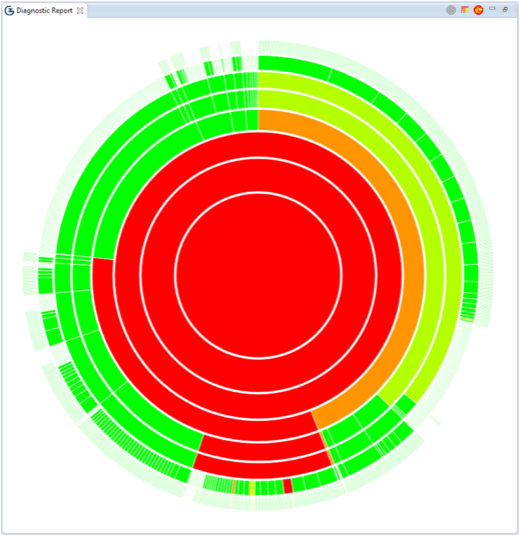
\includegraphics[width=0.5\textwidth]{barinel1.png}
    \caption{Sunburst visualization on Crowbar}
    \label{fig:crowbar-sunburst}
  \end{center}
\end{figure}

In addition to that information, this tool also shows us the component list sorted by fault likelihood.
